\documentclass[12pt,letterpaper]{article}

% Packages
\usepackage[margin=1in]{geometry}
\usepackage{graphicx}
\usepackage{amsmath}
\usepackage{amssymb}
\usepackage{booktabs}
\usepackage{siunitx}
\usepackage{float}
\usepackage{subcaption}
\usepackage{hyperref}
\usepackage{listings}
\usepackage{xcolor}
\usepackage{tikz}
\usepackage{circuitikz}
\usepackage{fancyhdr}

% Page formatting
\pagestyle{fancy}
\fancyhf{}
\lhead{8-bit Adder}
\rfoot{\thepage}

% Hyperref setup
\hypersetup{
    colorlinks=true,
    linkcolor=blue,
    filecolor=magenta,      
    urlcolor=cyan,
    citecolor=blue,
}

% Code listing style
\lstset{
    basicstyle=\ttfamily\small,
    breaklines=true,
    frame=single,
    numbers=left,
    numberstyle=\tiny,
}

% Title information
\title{\textbf{8-bit Ripple Carry Adder} \\}
       \vspace{0.5cm}

\author{Krishna Karthikeya Chemudupati \\ Adithya Selvakumar \\}
\date{November 11, 2025}

\begin{document}

\maketitle
\thispagestyle{empty}

\vspace{1cm}

\begin{abstract}
This report presents the design, implementation, and optimization of an 8-bit ripple-carry adder (RCA) in 45nm CMOS technology using Cadence design tools. The design includes a baseline implementation using minimum-sized transistors and an optimized version targeting at least 25\% delay improvement. The report details the circuit architecture, verification methodology, performance metrics (delay, active energy, and leakage energy), and the optimization process. The final optimized design achieves XX\% delay improvement over the baseline while maintaining correct logical functionality.
\end{abstract}

\newpage

\tableofcontents

\newpage

\section{Introduction}
\label{sec:introduction}

% TODO: Brief introduction to the project objectives and scope
% - Purpose of designing an 8-bit ripple-carry adder
% - Importance in digital system design
% - Overview of baseline and optimized designs
% - Report organization

\subsection{Project Objectives}

\subsection{Design Specifications}

\subsection{Report Organization}

\section{Background and Theory}
\label{sec:background}

% TODO: Theoretical foundation for adder design
% - Binary addition fundamentals
% - Full adder operation
% - Ripple-carry architecture

\subsection{Binary Addition}

\subsection{Full Adder Logic}

The full adder takes three inputs (A, B, Carry\_in) and produces two outputs (Sum, Carry\_out):

\begin{align}
\text{Sum} &= A \oplus B \oplus C_{in} \\
\text{Carry}_{out} &= AB + AC_{in} + BC_{in}
\end{align}

\subsection{Ripple-Carry Adder Architecture}

\subsection{Critical Path Analysis}

\section{Baseline Design}
\label{sec:baseline}

% TODO: Complete description of baseline design
% - Circuit topology selection
% - Transistor-level schematics
% - Design rationale

\subsection{Design Approach}

\subsection{Full Adder Bit-Slice Design}

\subsubsection{Circuit Topology}

\subsubsection{Transistor-Level Schematic}

% TODO: Include schematic figure
\begin{figure}[H]
    \centering
    % \includegraphics[width=0.8\textwidth]{figures/baseline_bitslice.png}
    \caption{Baseline full adder bit-slice schematic (minimum-sized transistors)}
    \label{fig:baseline_bitslice}
\end{figure}

\subsubsection{Design Parameters}

\begin{itemize}
    \item Technology: 45nm CMOS
    \item Supply Voltage: $V_{dd} = 1.2V$
    \item Transistor Sizes: Minimum ($W_{min}/L_{min}$)
    \item Logic Discipline: CMOS
\end{itemize}

\subsection{8-bit Ripple-Carry Adder Architecture}

\subsubsection{Cascading Strategy}

\subsubsection{Complete Adder Schematic}

% TODO: Include 8-bit adder schematic
\begin{figure}[H]
    \centering
    % \includegraphics[width=0.9\textwidth]{figures/baseline_8bit.png}
    \caption{Complete 8-bit ripple-carry adder - baseline design}
    \label{fig:baseline_8bit}
\end{figure}

\section{Functional Verification}
\label{sec:verification}

% TODO: Describe verification methodology and results

\subsection{Verification Methodology}

\subsection{Test Case Selection}

The following test cases were selected to exercise critical operating modes of the ripple-carry adder:

\begin{table}[H]
\centering
\caption{Test cases for functional verification}
\label{tab:test_cases}
\begin{tabular}{@{}cccccl@{}}
\toprule
\textbf{Test} & \textbf{A (dec)} & \textbf{B (dec)} & \textbf{Cin} & \textbf{Expected} & \textbf{Purpose} \\
\textbf{\#} & & & & \textbf{Sum/Cout} & \\
\midrule
1 & 255 & 1 & 0 & 0/1 & Full carry propagation \\
2 & 0 & 0 & 0 & 0/0 & Quiescent state \\
3 & 255 & 255 & 0 & 254/1 & Maximum output \\
4 & 170 & 85 & 0 & 255/0 & No carry propagation \\
5 & 3 & 1 & 0 & 4/0 & Partial carry \\
\bottomrule
\end{tabular}
\end{table}

\subsubsection{Test 1: Full Carry Propagation (A=255, B=1)}

\begin{table}[H]
\centering
\caption{Test 1 - Detailed bit-level verification}
\begin{tabular}{@{}ccccccccc|c@{}}
\toprule
\textbf{Bit} & \textbf{7} & \textbf{6} & \textbf{5} & \textbf{4} & \textbf{3} & \textbf{2} & \textbf{1} & \textbf{0} & \textbf{Cout} \\
\midrule
A & 1 & 1 & 1 & 1 & 1 & 1 & 1 & 1 & - \\
B & 0 & 0 & 0 & 0 & 0 & 0 & 0 & 1 & - \\
\midrule
Expected S & 0 & 0 & 0 & 0 & 0 & 0 & 0 & 0 & 1 \\
Simulated S & 0 & 0 & 0 & 0 & 0 & 0 & 0 & 0 & 1 \\
\bottomrule
\end{tabular}
\end{table}

% TODO: Include waveform
\begin{figure}[H]
    \centering
    % \includegraphics[width=0.9\textwidth]{figures/test1_waveform.png}
    \caption{Test 1 simulation waveform showing full carry propagation}
    \label{fig:test1}
\end{figure}

\subsubsection{Test 2: Zero Case (A=0, B=0)}

% TODO: Similar structure for remaining tests

\subsubsection{Test 3: Maximum Output (A=255, B=255)}

\subsubsection{Test 4: No Carry Propagation (A=170, B=85)}

\subsubsection{Test 5: Partial Carry (A=3, B=1)}

\subsection{Verification Results Summary}

% TODO: Summary table showing pass/fail for all tests

\section{Baseline Performance Metrics}
\label{sec:baseline_metrics}

% TODO: Detailed measurement methodology and results

\subsection{Delay Measurement}

\subsubsection{Measurement Setup}

\begin{itemize}
    \item Input Drive: Equivalent to one adder input capacitance
    \item Output Load: Equivalent to one adder input capacitance
    \item Worst-Case Input: A=255, B=1 (full carry propagation)
\end{itemize}

\subsubsection{Delay Results}

\begin{table}[H]
\centering
\caption{Baseline delay measurements}
\label{tab:baseline_delay}
\begin{tabular}{@{}lcc@{}}
\toprule
\textbf{Parameter} & \textbf{Value} & \textbf{Units} \\
\midrule
Worst-case delay ($t_{pd}$) & XX.XX & ns \\
Input to Sum[0] delay & XX.XX & ns \\
Input to Sum[7] delay & XX.XX & ns \\
Input to Cout delay & XX.XX & ns \\
\bottomrule
\end{tabular}
\end{table}

% TODO: Include delay measurement waveform
\begin{figure}[H]
    \centering
    % \includegraphics[width=0.9\textwidth]{figures/baseline_delay.png}
    \caption{Baseline design delay measurement (worst-case path)}
    \label{fig:baseline_delay}
\end{figure}

\subsection{Active Energy Measurement}

\subsubsection{Maximum Switching Energy Case}

Test condition: All inputs switch from $0 \rightarrow 1$

\begin{equation}
E_{active,max} = \int_{t_{start}}^{t_{end}} V_{dd} \cdot I_{dd}(t) \, dt = \text{XX.XX fJ}
\end{equation}

\begin{figure}[H]
    \centering
    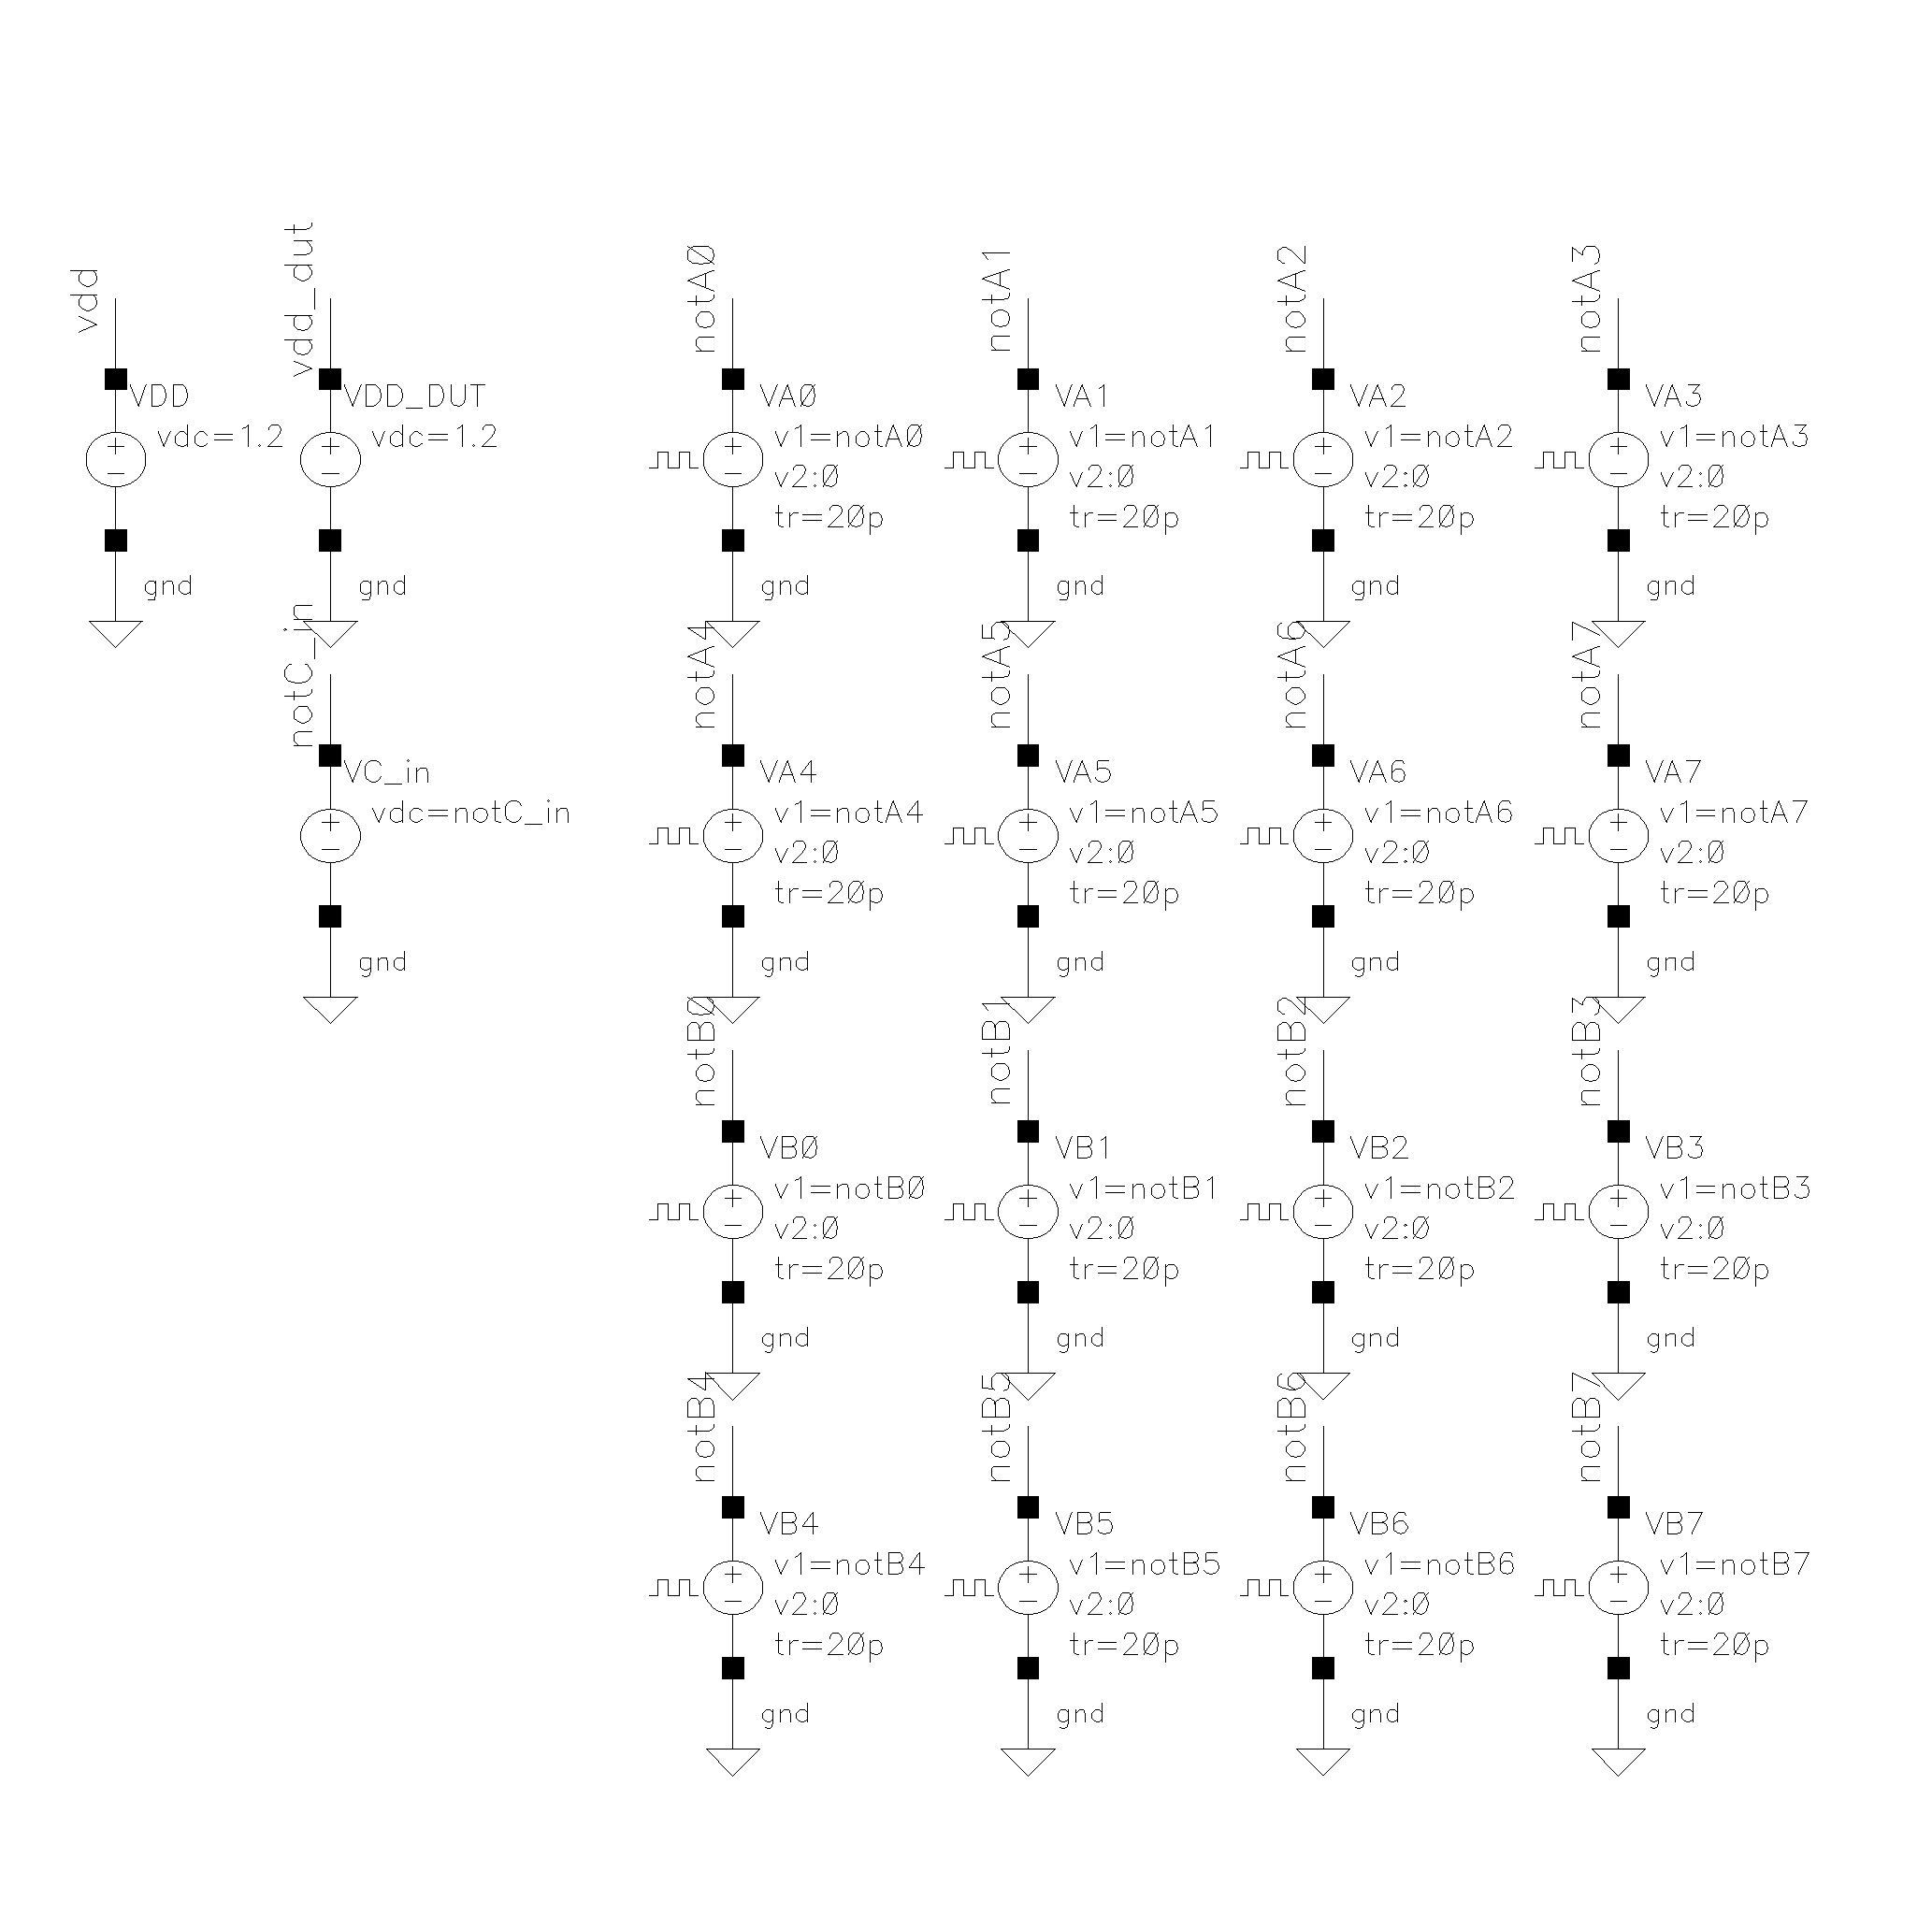
\includegraphics[width=\linewidth]{writeup//figures//baseline//active_energy/max_switching_energy_inputs.png}
    \caption{Enter Caption}
\end{figure}

\begin{figure}[H]
    \centering
    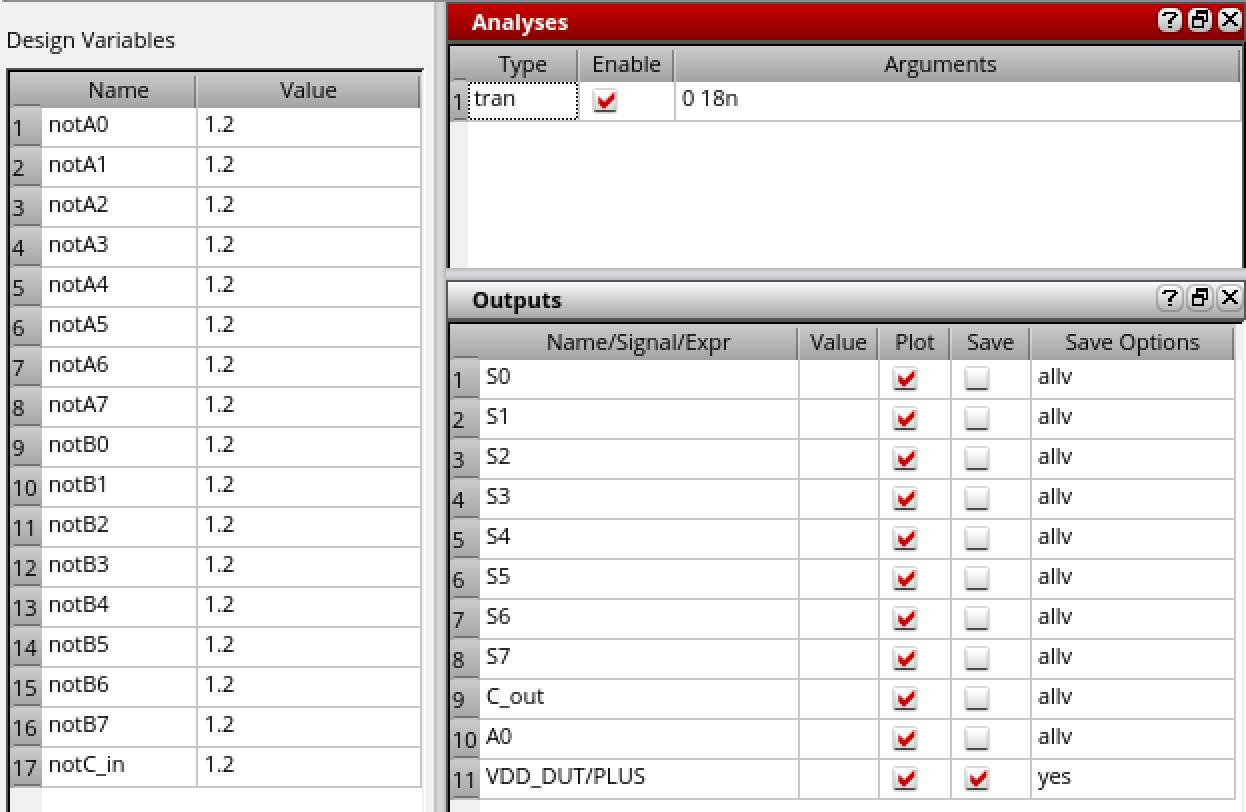
\includegraphics[width=\linewidth]{writeup//figures//baseline//active_energy/max_switching_energy_adel.png}
    \caption{Enter Caption}
\end{figure}

\begin{figure}[H]
    \centering
    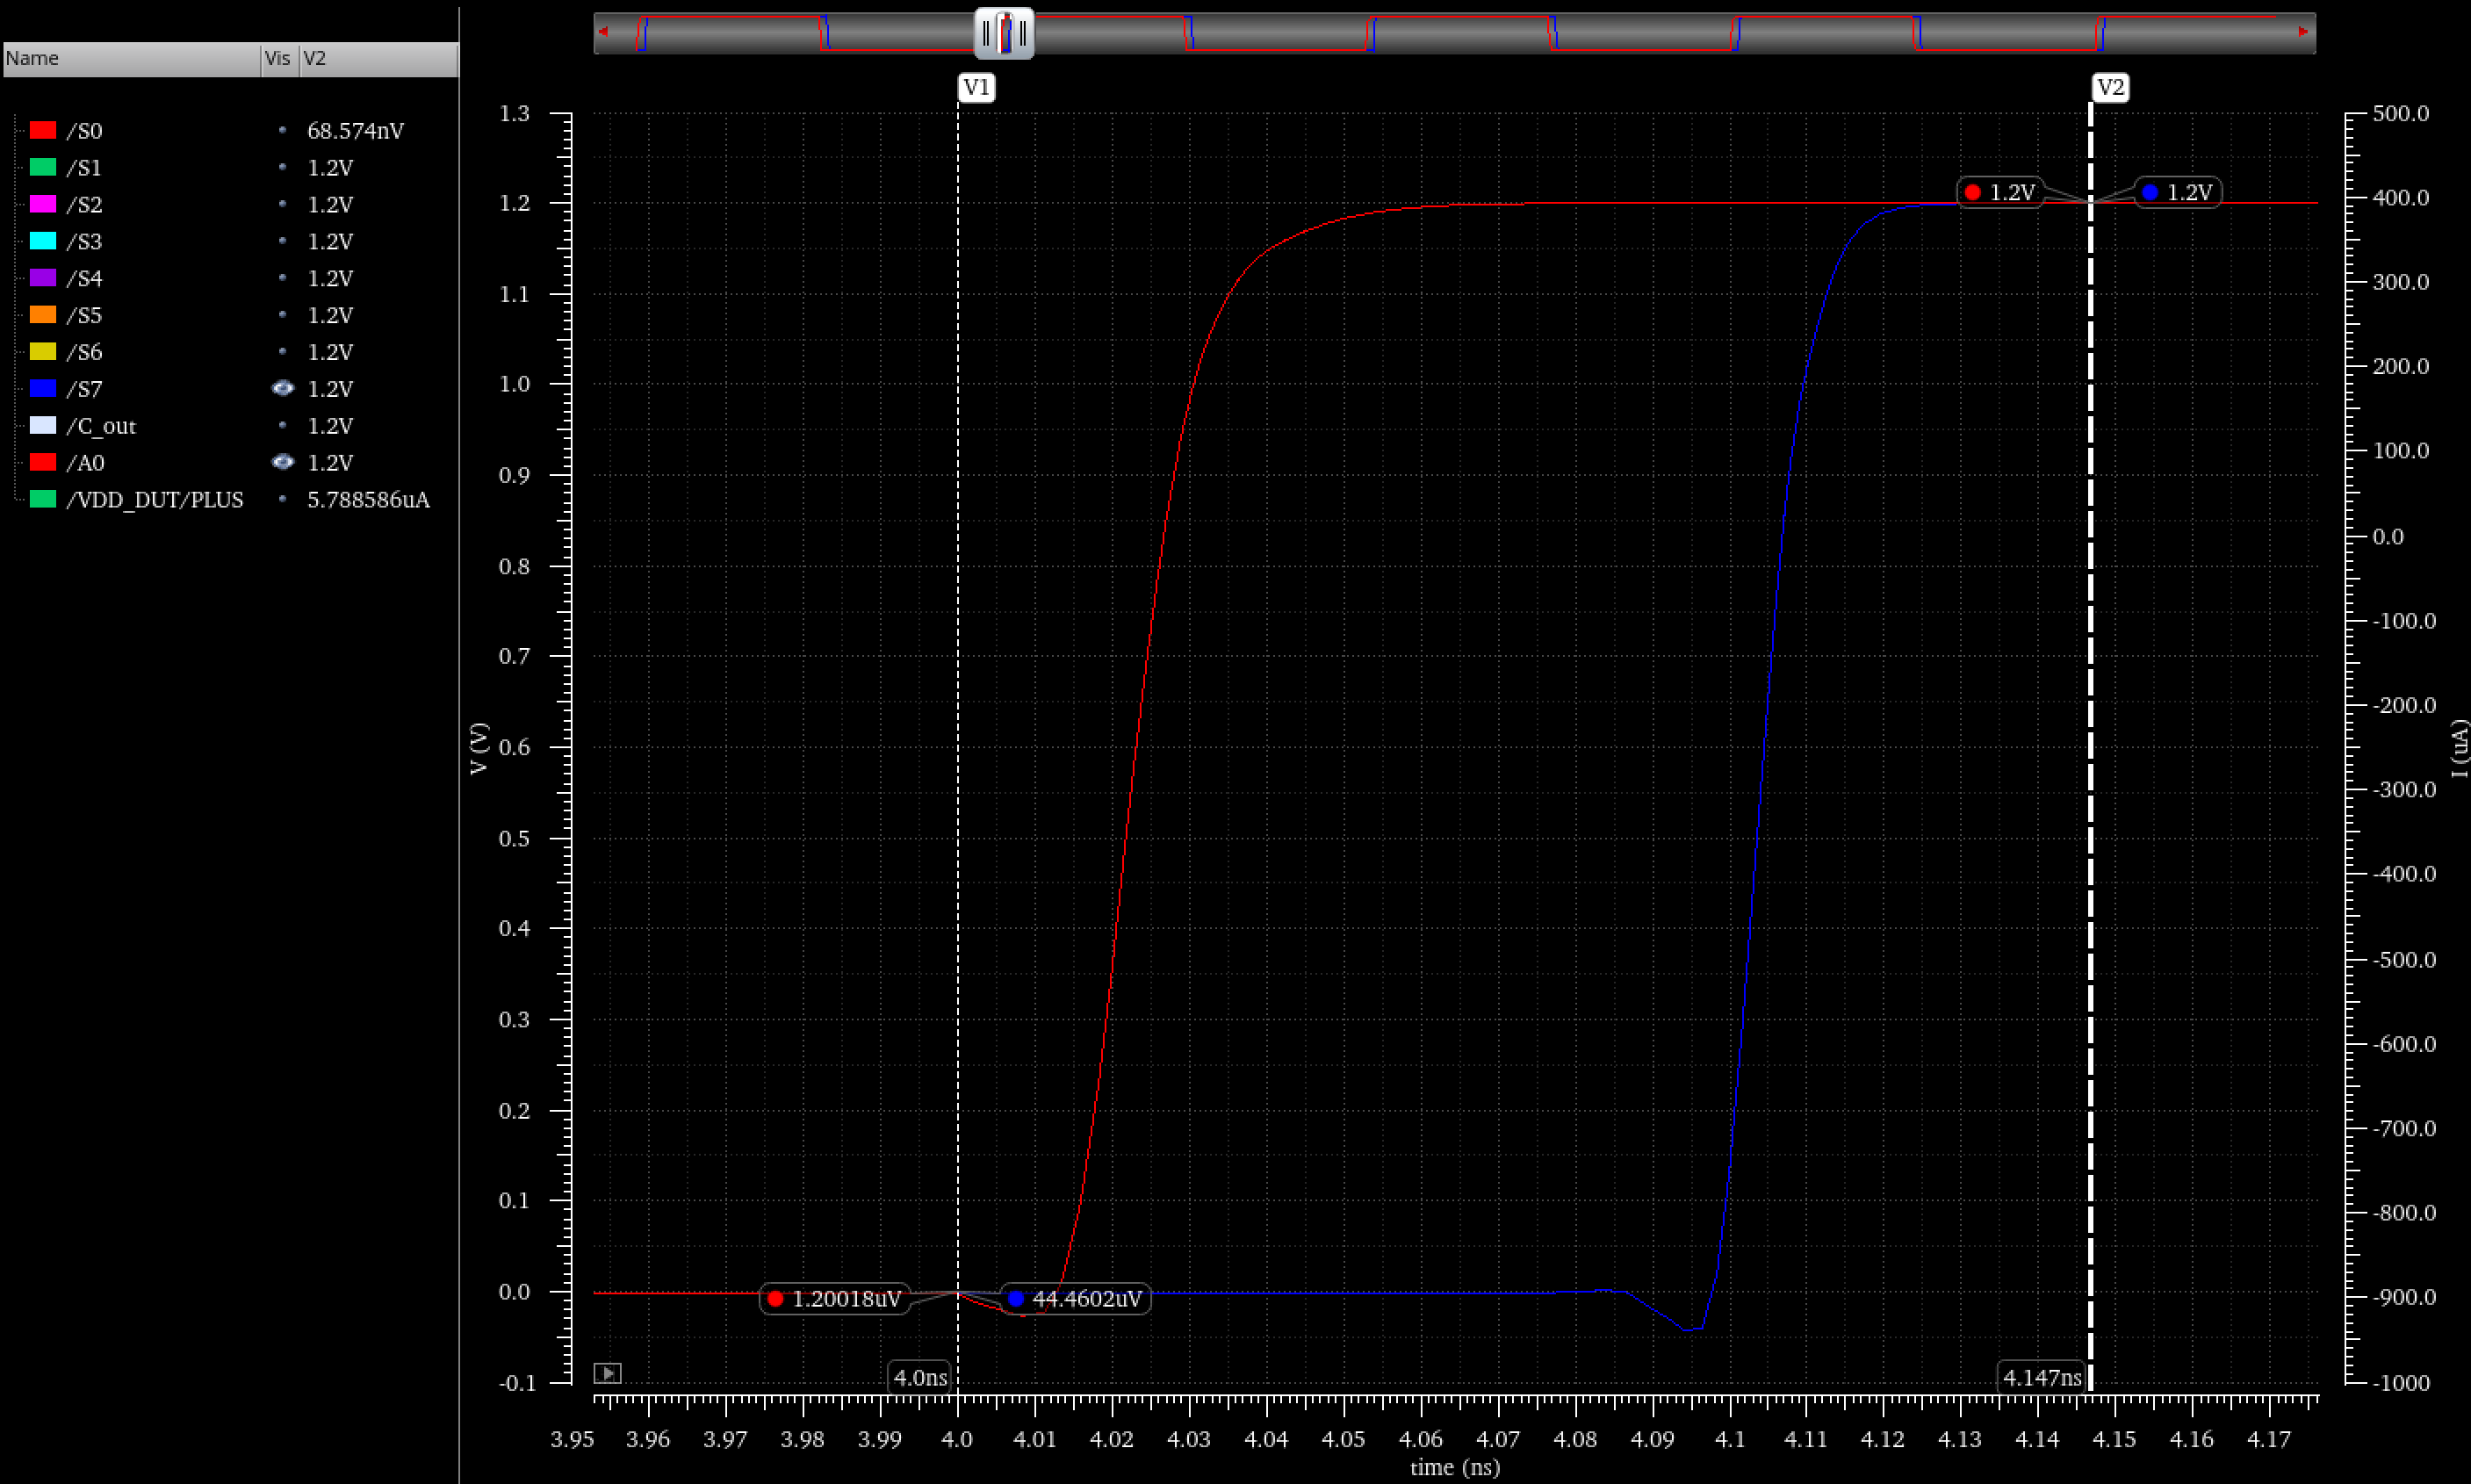
\includegraphics[width=1\linewidth]{writeup//figures//baseline//active_energy/max_switching_energy_signals.png}
    \caption{Enter Caption}
\end{figure}

\begin{figure}[H]
    \centering
    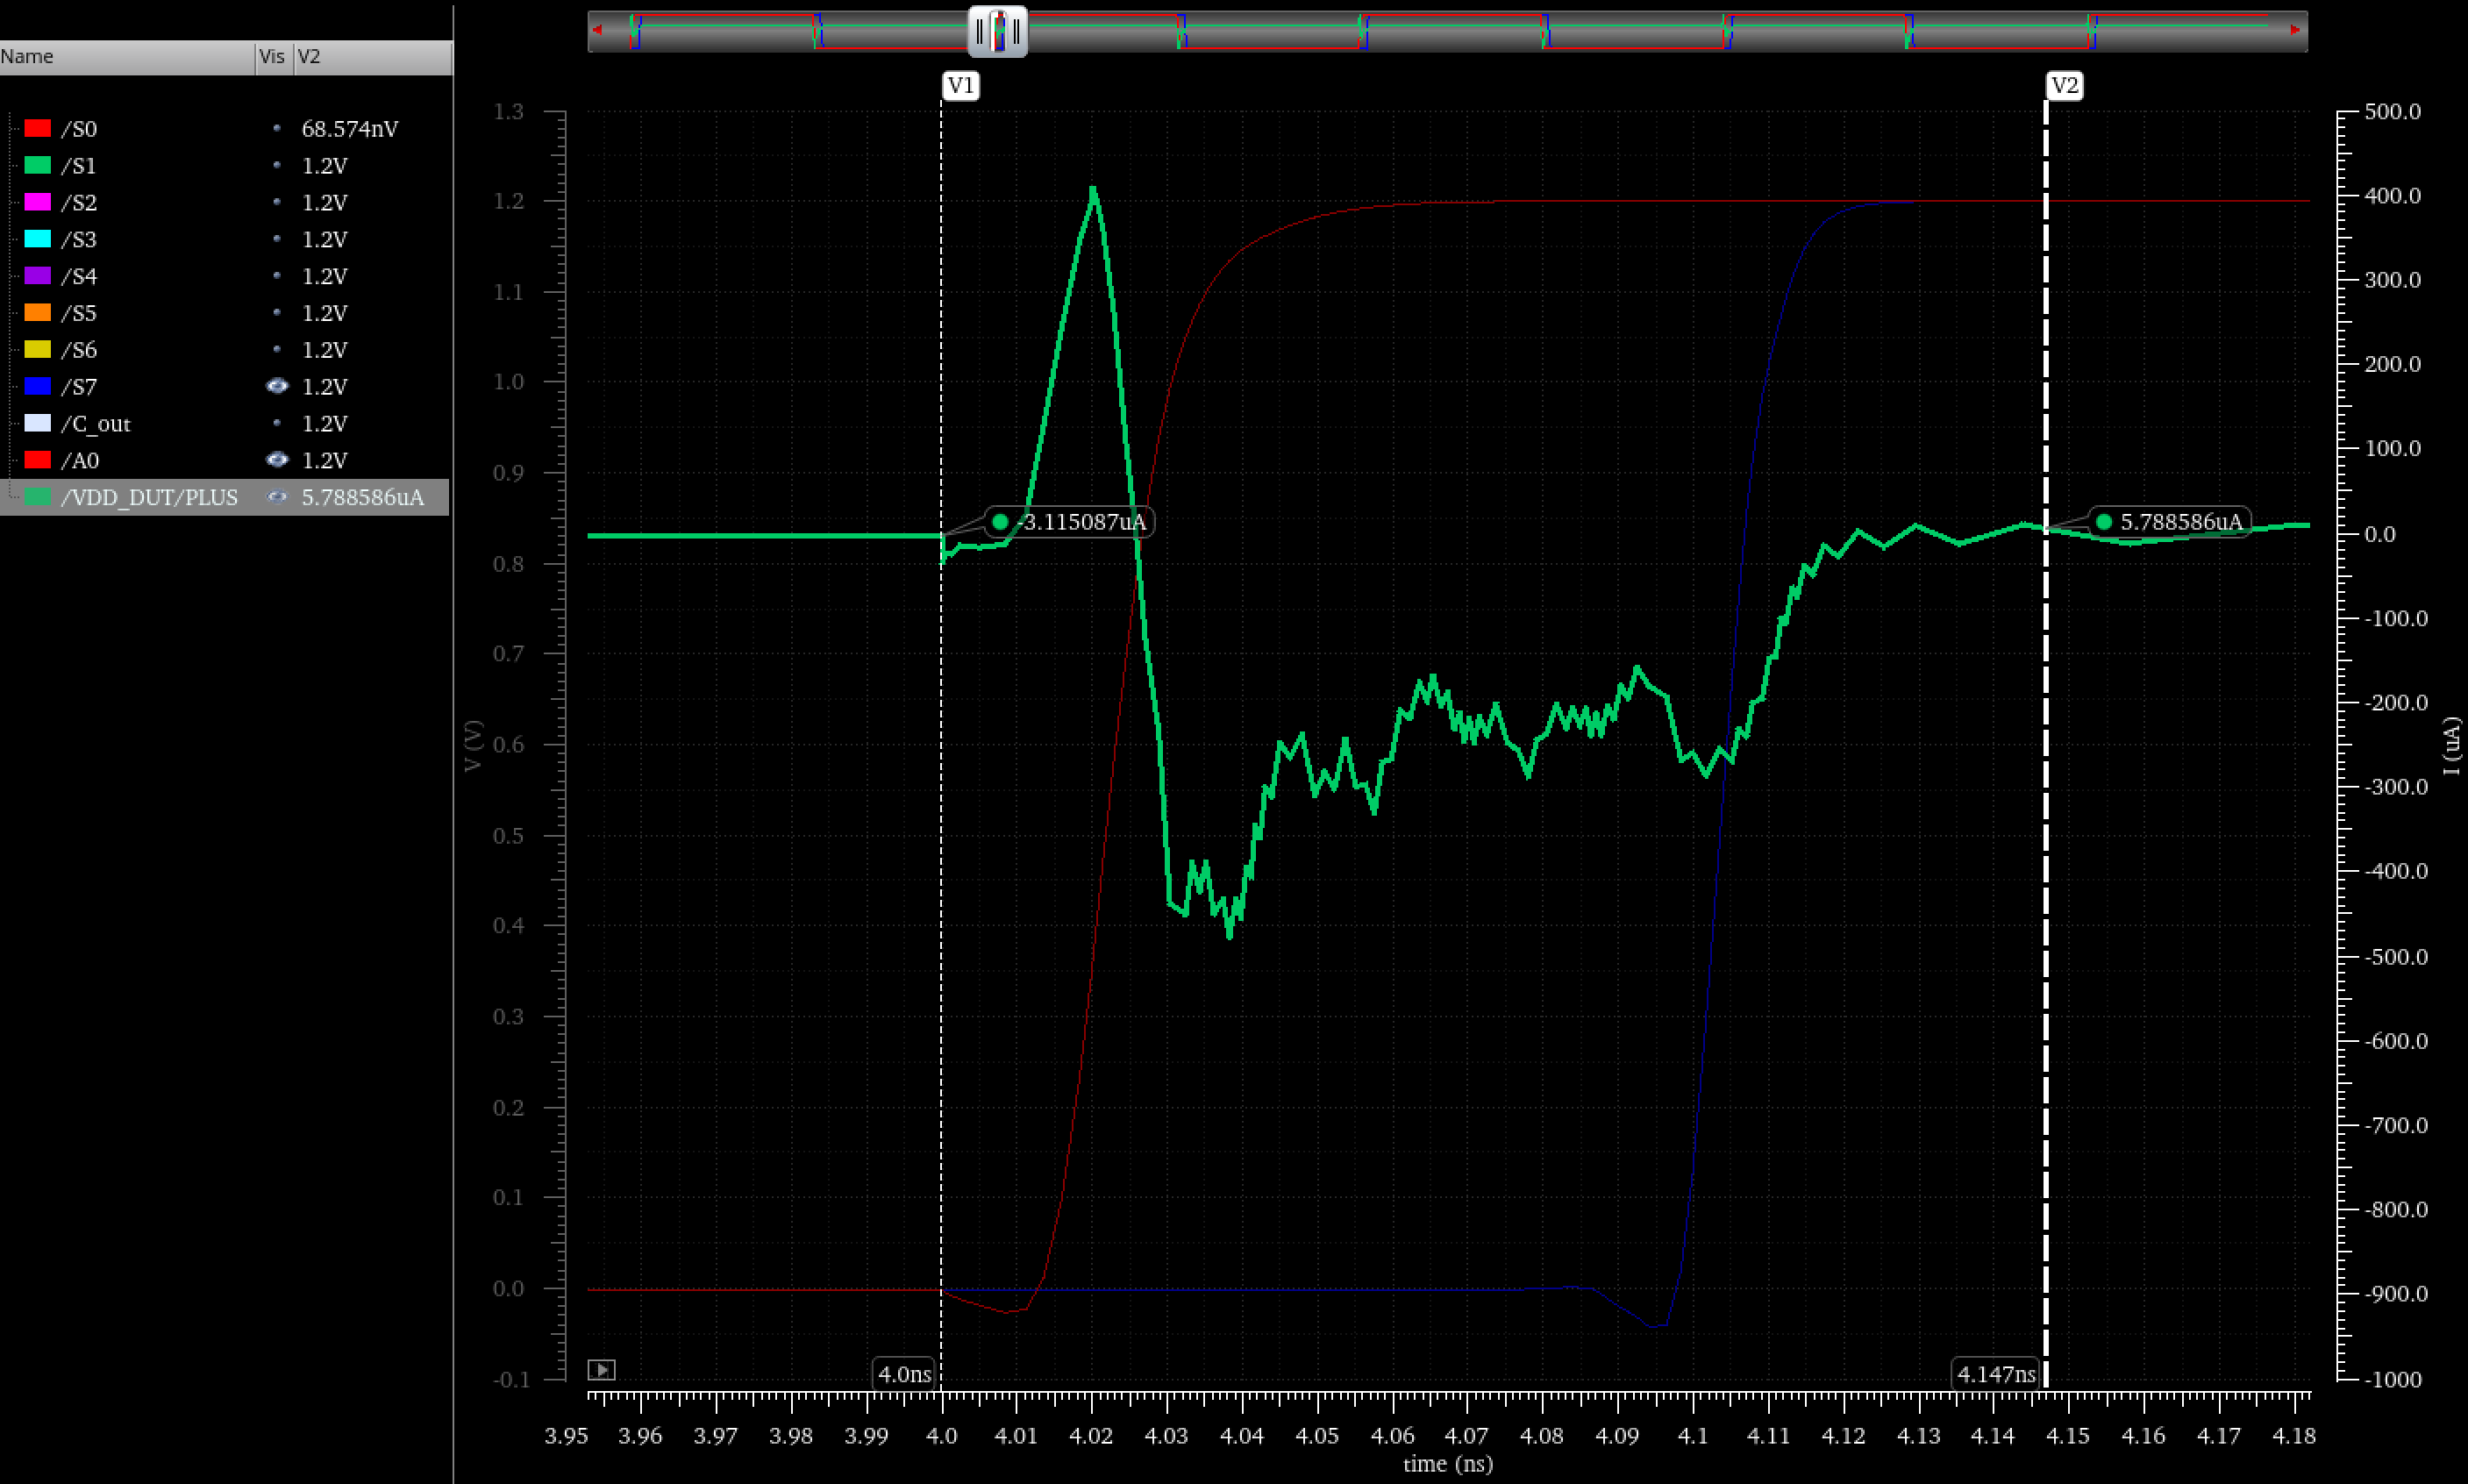
\includegraphics[width=1\linewidth]{writeup//figures//baseline//active_energy/max_switching_energy_current.png}
    \caption{Enter Caption}
\end{figure}

\begin{figure}[H]
    \centering
    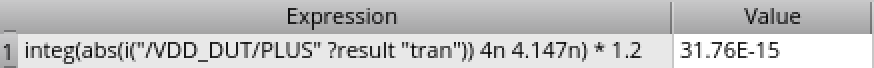
\includegraphics[width=0.5\linewidth]{writeup//figures//baseline//active_energy/max_switching_energy_value.png}
    \caption{Enter Caption}
\end{figure}

\subsubsection{Average Switching Energy Case}

Test condition: Half the inputs switch from $0 \rightarrow 1$

\begin{equation}
E_{active,avg} = \text{XX.XX fJ}
\end{equation}

\begin{table}[H]
\centering
\caption{Baseline active energy measurements}
\label{tab:baseline_active_energy}
\begin{tabular}{@{}lcc@{}}
\toprule
\textbf{Case} & \textbf{Energy} & \textbf{Units} \\
\midrule
Maximum switching & XX.XX & fJ \\
Average switching & XX.XX & fJ \\
\bottomrule
\end{tabular}
\end{table}

\subsection{Leakage Energy Measurement}

\subsubsection{Leakage Power Calculation}

For static inputs over one delay period:

\begin{equation}
E_{leakage} = P_{leakage} \cdot t_{pd}
\end{equation}

\subsubsection{Maximum Leakage Case}

Input condition: [Describe the input combination that gives maximum leakage]

Justification: [Explain why this gives maximum leakage based on transistor states]

\subsubsection{Minimum Leakage Case}

Input condition: [Describe the input combination that gives minimum leakage]

Justification: [Explain why this gives minimum leakage]

\begin{table}[H]
\centering
\caption{Baseline leakage energy measurements}
\label{tab:baseline_leakage}
\begin{tabular}{@{}lcc@{}}
\toprule
\textbf{Case} & \textbf{Energy} & \textbf{Units} \\
\midrule
Maximum leakage & XX.XX & fJ \\
Minimum leakage & XX.XX & fJ \\
\bottomrule
\end{tabular}
\end{table}

\subsection{Baseline Metrics Summary}

\begin{table}[H]
\centering
\caption{Complete baseline design metrics}
\label{tab:baseline_summary}
\begin{tabular}{@{}lcc@{}}
\toprule
\textbf{Metric} & \textbf{Value} & \textbf{Units} \\
\midrule
Delay ($t_{pd}$) & XX.XX & ns \\
Active Energy (max) & XX.XX & fJ \\
Active Energy (avg) & XX.XX & fJ \\
Leakage Energy (max) & XX.XX & fJ \\
Leakage Energy (min) & XX.XX & fJ \\
\bottomrule
\end{tabular}
\end{table}

\section{Design Optimization}
\label{sec:optimization}

% TODO: Describe the optimization process and rationale

\subsection{Optimization Strategy}

\subsubsection{Design Space Exploration}

List of optimization techniques considered:
\begin{itemize}
    \item Transistor sizing
    \item Gate topology modifications
    \item Carry chain polarity optimization
    \item Logic discipline changes (CMOS, Pass-transistor, etc.)
    \item Supply voltage scaling
\end{itemize}

\subsection{Critical Path Analysis}

% TODO: Analyze the critical path and identify bottlenecks

\subsection{Optimization Iterations}

\subsubsection{Iteration 1: [Description]}

% TODO: Document each major optimization iteration
% - What was changed
% - Why it was expected to help
% - Hand analysis or simulation results
% - Decision to keep or reject

\subsubsection{Iteration 2: [Description]}

\subsubsection{Iteration N: [Description]}

\subsection{Design Trade-offs}

% TODO: Discuss trade-offs between delay, energy, area, complexity

\section{Optimized Design}
\label{sec:optimized}

% TODO: Complete description of final optimized design

\subsection{Final Design Architecture}

\subsection{Optimized Bit-Slice Design}

\subsubsection{Circuit Modifications}

\subsubsection{Transistor Sizing Strategy}

% TODO: Include optimized schematic
\begin{figure}[H]
    \centering
    % \includegraphics[width=0.8\textwidth]{figures/optimized_bitslice.png}
    \caption{Optimized full adder bit-slice schematic}
    \label{fig:optimized_bitslice}
\end{figure}

\subsection{Complete Optimized Adder}

% TODO: Include complete optimized 8-bit adder schematic
\begin{figure}[H]
    \centering
    % \includegraphics[width=0.9\textwidth]{figures/optimized_8bit.png}
    \caption{Complete 8-bit ripple-carry adder - optimized design}
    \label{fig:optimized_8bit}
\end{figure}

\section{Optimized Design Performance}
\label{sec:optimized_metrics}

% TODO: Performance measurements for optimized design
% Use same structure as baseline metrics section

\subsection{Delay Measurement}

\begin{table}[H]
\centering
\caption{Optimized delay measurements}
\label{tab:optimized_delay}
\begin{tabular}{@{}lcc@{}}
\toprule
\textbf{Parameter} & \textbf{Value} & \textbf{Units} \\
\midrule
Worst-case delay ($t_{pd}$) & XX.XX & ns \\
Input to Sum[0] delay & XX.XX & ns \\
Input to Sum[7] delay & XX.XX & ns \\
Input to Cout delay & XX.XX & ns \\
\bottomrule
\end{tabular}
\end{table}

\subsection{Active Energy Measurement}

\begin{table}[H]
\centering
\caption{Optimized active energy measurements}
\label{tab:optimized_active_energy}
\begin{tabular}{@{}lcc@{}}
\toprule
\textbf{Case} & \textbf{Energy} & \textbf{Units} \\
\midrule
Maximum switching & XX.XX & fJ \\
Average switching & XX.XX & fJ \\
\bottomrule
\end{tabular}
\end{table}

\subsection{Leakage Energy Measurement}

\begin{table}[H]
\centering
\caption{Optimized leakage energy measurements}
\label{tab:optimized_leakage}
\begin{tabular}{@{}lcc@{}}
\toprule
\textbf{Case} & \textbf{Energy} & \textbf{Units} \\
\midrule
Maximum leakage & XX.XX & fJ \\
Minimum leakage & XX.XX & fJ \\
\bottomrule
\end{tabular}
\end{table}

\subsection{Optimized Metrics Summary}

\begin{table}[H]
\centering
\caption{Complete optimized design metrics}
\label{tab:optimized_summary}
\begin{tabular}{@{}lcc@{}}
\toprule
\textbf{Metric} & \textbf{Value} & \textbf{Units} \\
\midrule
Delay ($t_{pd}$) & XX.XX & ns \\
Active Energy (max) & XX.XX & fJ \\
Active Energy (avg) & XX.XX & fJ \\
Leakage Energy (max) & XX.XX & fJ \\
Leakage Energy (min) & XX.XX & fJ \\
\bottomrule
\end{tabular}
\end{table}

\section{Performance Comparison}
\label{sec:comparison}

% TODO: Side-by-side comparison of baseline vs optimized

\subsection{Metrics Comparison}

\begin{table}[H]
\centering
\caption{Baseline vs. Optimized design comparison}
\label{tab:comparison}
\begin{tabular}{@{}lcccc@{}}
\toprule
\textbf{Metric} & \textbf{Baseline} & \textbf{Optimized} & \textbf{Improvement} & \textbf{Units} \\
\midrule
Delay & XX.XX & XX.XX & XX.XX\% & ns \\
Active Energy (max) & XX.XX & XX.XX & XX.XX\% & fJ \\
Active Energy (avg) & XX.XX & XX.XX & XX.XX\% & fJ \\
Leakage Energy (max) & XX.XX & XX.XX & XX.XX\% & fJ \\
Leakage Energy (min) & XX.XX & XX.XX & XX.XX\% & fJ \\
\bottomrule
\end{tabular}
\end{table}

\subsection{Delay Improvement Analysis}

Percentage improvement in delay:
\begin{equation}
\text{Improvement} = \frac{t_{pd,baseline} - t_{pd,optimized}}{t_{pd,baseline}} \times 100\% = \text{XX.XX\%}
\end{equation}

\subsection{Energy Trade-offs}

% TODO: Discuss any energy penalties incurred for delay improvement

\subsection{Graphical Comparison}

% TODO: Include bar charts or other visualizations
\begin{figure}[H]
    \centering
    % \includegraphics[width=0.8\textwidth]{figures/comparison_chart.png}
    \caption{Baseline vs. Optimized performance comparison}
    \label{fig:comparison}
\end{figure}

\section{Discussion}
\label{sec:discussion}

% TODO: Interpret results and discuss findings

\subsection{Design Insights}

\subsection{Optimization Effectiveness}

\subsection{Limitations and Future Work}

\section{Conclusion}
\label{sec:conclusion}

% TODO: Summarize the project and key findings
% - Successfully designed and verified 8-bit RCA
% - Achieved XX% delay improvement
% - Key optimization techniques that were effective
% - Final thoughts

\end{document}